\chapter{Probability}

\begin{multicols}{2}[\subsubsection*{Contents of this chapter}]
   \printcontents{}{1}{\setcounter{tocdepth}{2}}
\end{multicols}


\section{Interpretations and Definitions of Probability}

\subsection{Naive and Non-Naive Definitions of Probability}
Probability courses typically start with what \citeasnoun{blitzstein2019introduction} calls the \textit{naive} definition of probability, which is to look at the fraction of the event space that corresponds to a particular event. This works well for combinatorial type of probability problems, such as the likely outcome of dice throws. The dichotomy below is from \citeasnoun{blitzstein2019introduction}.

\subsubsection{Naive Probability}
The event space $S$ consists of a collection of equally likely outcomes. The actual outcome $s_{actual} \in S$. The probability of an outcome in a subset $A\subseteq S$, $P(s_{actual}\in A)$ corresponds to the fraction of events in $A$ out of $S$.

\begin{equation}
P_{naive}(A) = \frac{|A|}{|S|} = \frac{\mathrm{number of outcomes favorable to A}}{\mathrm{total number of outcomes in S}}
\end{equation}

This approach runs into trouble when the outcomes in $|A|$ are not equally likely, or if the sample space is infinite, i.e. $|S|=\infty$.


\subsubsection{Non-Naive Definition of Probability}
A probability space consists of a sample space $S$ in addition to a \textit{probability function}. The job of the probability function is to take an event $A\subseteq S$ and map it to a number between $0$ and $1$. I.e.  $P: S \rightarrow [0,1]$.

The function $P$ must satisfy:

\begin{itemize}
\item P(\empty) = 0, P(S) = 1
\item If $A_1, A_2,...$ are \textit{disjoint} events, then: \begin{equation}P\left(\bigcup^{\infty}_{j=1}A_j \right) = \sum_{j=1}^{\infty}P(A_j)\end{equation}
\end{itemize}

In other words, all you need to work with probability is a set of possible outcomes $S$ and some function to apply to parts of that set.

\subsection{Frequentist Probability}
The \textit{frequentist} interpretation of probability is that it represents the frequency of an outcome of a particular experiment upon running the experiment many times. On one hand, this view on probability is arguably empirically grounded. On the other hand it relies on the impractical notion of identically repeating something a large number of times. 

\subsection{Bayesian Probability}
The \textit{Bayesian} view on probability is that it represents a degree of belief in a particular outcome. On one hand, this implies a degree of subjectivity. On the other hand, this notion of probability is much more broadly applicable, because it does not require repeatable experiments. It also permits the introduction of subjective biases through priors.

I'm not sure whether the supposed "battle" between frequentists and Bayesians has ever been of any consequence for me. Also, the frequentist perspective strikes me as inherently contradictory, because supposed empirical proof can strictly speaking never be practically delivered.

In practice, it seems that frequentist approaches tend to be structured around parametrization of solutions in terms of summary statistics, while Bayesians have a tendency to approach problems in terms of full probability distributions. Social scientists seem to be leaning towards frequentist methods, while physicists and engineers seem to be more interested in Bayesian data analysis. 

I suspect that an additional source of bias is that frequentist methods tend to be computationally lighter and that many standard accepted recipes exist for common problems. In contrast, Bayesian approaches are usually derived ad-hoc in the context of a particular problem.

\subsection{Measure Theoretic Probability}
The modern approach to probability is rooted in measure theory. In that context:

\begin{itemize}
\item The \textit{sample space} is a measurable set
\item An \textit{event} is a measurable set; a subset of the sample space.
\item A \textit{random variable} is a measurable function on the sample space.
\item The \textit{expectation} of a random variable is its integral with respect to the probability measure.
\end{itemize}


	
\section{Functions of Random Variables, Derived Distributions}

(This section needs revision)

I find changes of variables to be the easiest to understand by writing down a joint probability distribution using a delta function to express the conditional probability for the new variables based on the old variables. The next step is to perform a change of variables in the delta function, and integrate. The delta function means that the relationship between the old and the new variables is deterministic. If the relationship is non-deterministic you can use whatever expression for the conditional probability is appropriate.

Let's say that you want to know the probability distribution of the function $\vec{u} = \mathbf{H}(\vec{x})$ of some random variable $\vec{x}$ for which the probability distribution is known.

I personally find it least confusing to approach this problem by thinking about the joint probability distribution, and then obtaining $p(\vec{u})$ through marginalization:

\begin{equation}
p(\vec{u}) = \int dx^n p(\vec{x},\vec{u}) = \int dx^n p_x(\vec{x}) p_u(\vec{u}|\vec{x})
\end{equation}

Since $\vec{u}$ is a deterministic function of $\vec{x}$, the conditional probabiltiy $p_u(\vec{u}|\vec{x}) = \delta(\vec{u} - \mathbf{H}(\vec{x}))$. Explicitly:

\begin{equation}
p(\vec{u}) = \int dx^n p_x(\vec{x}) \delta(\vec{u} - \mathbf{H}(\vec{x}))
\end{equation}

What this does, is to integrate over all the points $p_x(\vec{x})$ where the argument of the delta function is zero. The important thing is that care needs to be taken when the argument of the delta function is itself a function. In that case, a change of variables has to be performed, so that this is no longer the case. On wikipedia, this is done by defining the new variable $du = |\frac{d}{dx}g(x)|dx$, from which follows:

\begin{equation}
\delta(g(x)) = \sum_{x_0} \frac{\delta(x-x_0)}{|g'(x_0)|}
\end{equation}

Where it is necessary to sum over each point $x_0$ for which $g(x_0) = 0$.

Which makes sense. Except, if you rewrite in terms of the new variable, you get an expression that does not strike me as necessarily the same:

\begin{equation}
\int f(x) \delta(g(x))dx = \sum_{n}\int f(g_n^{-1}(u)) \delta(u) \left|\frac{d}{du}g^{-1}(u)\right|du
\end{equation}

Where the sum $n$ is over all functions $g_n^{-1}$ that satisfy $g(g_n^{-1}(u)) = u$. For example, if $u = g(x) = sin(x)$ then $g_n^{-1} = asin(u) + n2\pi$, for any integer $n$. I feel more comfortable with the second path. The answer to my confusion is most likely the inverse function theorem (cf. section \ref{sec:inverse_function_theorem}). In other words: this section needs revision! But hey, I flagged it.

Note that a delta function with a vector argument can be written as a product of the delta functions along each dimension.

Define a new set of variables $\vec{a} = \vec{u} - \mathbf{H}(\vec{x})$. It follows that $\vec{x} = \mathbf{H_n^{-1}}(\vec{u}-\vec{a})$ and the volume element $dx^n = \left| \frac{d}{d\vec{a}}\mathbf{H}_n^{-1}(\vec{u}-\vec{a})\right|da^n$. Here, $H^{-1}_n$ are all the functions that satisfy $\mathbf{H}(\mathbf{H}_n^{-1}(\vec{u})) = \vec{u}$. The integral becomes:

\begin{equation}
p(\vec{u}) = \int da^n p_x(\mathbf{H}^{-1}_n(\vec{u}-\vec{a}))\left| \frac{d}{d\vec{a}}\mathbf{H}_n^{-1}(\vec{u}-\vec{a})\right| \delta(\vec{a})
\end{equation}

At this point it is safe to evaluate the delta function integral. The result is:

\begin{equation}
p(\vec{u}) = p_x(\mathbf{H}^{-1}_n(\vec{u})\left| \frac{d}{d\vec{a}}\mathbf{H}_n^{-1}(\vec{u}-\vec{a})\right|_{(\vec{a}=0)}
\end{equation}

\subsection{Example: Sum of Random Variables}
If the map $\mathbf{H}$ is not bijective, for example because $\vec{u}$ has lower dimensionality than $\vec{x}$, then a bijective map can be artifically constructed by introducing additional variables that are then also marginalized out. For example, if the goal is to calculate the probability of measuring some sum of random variables $s$, then you can define:

\begin{equation}
u_0 = s - \sum(x_i)\\
u_1 = x_1\\
u_2 = x_2\\
\vdots\\
u_{(n-1)} = x_{n-1}
\end{equation}

The inverse is:

\begin{equation}
x_1 = u_1\\
x_2 = u_2\\
\vdots\\
x_n = s - u_0 - \sum_{i<n} x_i
\end{equation}

The argument in the delta function is transformed $\delta(s - \sum(x_i)) \rightarrow \delta(u_0)$. The determinant of the Jacobian $|J| = |\frac{d}{d\vec{u}} H^{-1}(\vec{u})|$ is given by $[\frac{d}{du_1} \mathbf{H^{-1}},\frac{d}{du_2} \mathbf{H^{-1}},...,\frac{d}{du_{n-1}} \mathbf{H^{-1}}]$. That's an $nxn$ matrix where the first row is all $-1$, the lower left is an $(n-1)x(n-1)$ identity matrix, and the lower right is a $(n-1)x1$ vector of 0s. The determinant is one. Consequently the probability distribution of measuring a sum $s$ is given by:

\begin{equation}
p(s)= \int dx^{n-1} p_x(x_1,x_2,x_3,...,s-\sum_{x<n}x_i)
\end{equation}

Which turns out to be the convolution when the variables are independent.

\subsection{Example: Lower Dimensional Random Variable}

This was already the case for the sum of several random variables, in which case the dimensionality of the problem was reduced from many to one. 

Consider the case many to fewer. Again, you just need to perform a change of variables. The new set of variables needs to have the same dimensionality as the old set of variables. The rest should follow pretty obviously. 

Linear example: $\vec{y} = \mathbf{M}\vec{x}$ where $y$ has 2 dimensions and $x$ has 3. 

Transform:

\begin{equation}
u_1 = y_1 - \vec{M_1}\cdot\vec{x}\\
u_2 = y_2 - \vec{M_2}\cdot\vec{x}\\
u_3 = x_3
\end{equation}

You can write this in terms of some invertible matrix $\mathbf{W} = [\mathbf{M},[0,0,1]]$ as $\vec{u} = \mathbf{W}\vec{x}$, so that $dx^n = |\mathbf{W}^{-1}|du^n|$. The integral is then:

\begin{equation}
p(y) = \int du^n p_x(\mathbf{W}^{-1}(\vec{y}-\vec{u}))\delta(u_1)\delta(u_2)|\mathbf{W}^{-1}|
\end{equation}

\section{Indicator Variables}

Indicator variables are useful devices that simplify probability calculations involving binary outcomes, namely wether the outcome lies in a certain region of event space or not. Specifically, they allow one to translate set expressions into algebraic expressions. 

Let $A\subseteq S$ be a subset of event space $S$ (ex. $A\equiv$ "it rains tomorrow"). Then the indicator variable $I_A$: 

\begin{equation}
I_A = \left\{\begin{array}{l} 1 \mathrm{\ if\ outcome\ in\ A}\\0 \mathrm{\ if\ outcome\ in\ A^c} \end{array}\right.
\end{equation}

Which means that:
\begin{equation}
\mathbb{E}(I_A) = 1\times p(A) + 0\times p(A^c)= p(A)
\end{equation}

To indicator variables for different events $A,B,C...$ can also be combined:
\begin{equation}
I_{A\cap B\cap C\cap ...} = I_A I_B I_C ...
\end{equation}

And indicator variables for the complement can be constructed trivially:
\begin{equation}
I_{A^c} = 1 - I_A
\end{equation}

Whenever accounting for complicated combinations of events becomes overwhelming, indicator variables are often a good approach.

\subsection{Example: The Party Problem}

The party problem is a typical interview question, so I will include the two easier problems that do not make use of indicator variables. (This version of my notes also still has bitterness included.)

There are $n$ drunk kids at a party that is presumably getting shut down by the fun police in Cambridge, MA. They (meaning the kids, presumably) grab their coats at random, and the problem is built around thinking about how many people wind up with the correct coat.

\subsubsection{Lame Interview Question 1: Every one finds their coat}
The common version of this problem asks "what is the probability that all of the kids wind up with the right coat". This is much easier than the general case. Imagine the list of party guests as a sequence $(1,2,3,4,...,n-1,n)$ and the coats they grab as a random permutation of that sequence, such as $\alpha = (6,1,40,21,9,...)_n$. There are $n!$ such permutations, and they are all equally likely. The probability of all guests getting the correct coat is the probability that the permutation happens to be the single correct one, i.e. $p(\alpha = (1,2,3,4,...,n-1,n)_n)$, which is the probality of one particular permutation, i.e. $p(\alpha = (1,2,3,4,...,n-1,n)_n) = \frac{1}{n!}$.

\subsubsection{Lame Interview Question 2: At least r people find their coat}
This is still pretty easy, because the permutations that are correct are easily counted. If at least $r$ coats are correctly assigned, then there are $\left(\begin{array}{l}n\\r\end{array}\right)$ ways of choosing wich of the $r$ people wind up with the right coat. Then, while the location of $r$ indices in the sequence is fixed, $n-r$ indices can be assigned arbitrarily.

The number of permutations where at least $r$ are assigned correctly are then:

\begin{equation}
\left(
\begin{array}{l}
n\\
r
\end{array}
\right)(n-r)!
\end{equation}

And the probability of at least $r$ people finding their coat is the number of permutations multiplied with the probability of an individual permutation (that is, $\frac{1}{n!}$):

\begin{equation}
p(\mathrm{\#\ correct} \geq r)=\left(
\begin{array}{l}
n\\
r
\end{array}
\right)\frac{(n-r)!}{n!} = \frac{1}{r!}
\end{equation}

Where $r\leq n$.

\subsubsection{Not lame: Exactly r people find their coat}
So, then, what's the probability that exactly nobody finds their coat? What's the probability that 2 people find their coat but nobody else does? What's the probability that $r$ out of $n$ people find their coat? After thinking quickly on your feet for two seconds, you realize that the answer is obviously:

\begin{equation}
p(\mathrm{\#\ correct} = r) = \frac{1}{r!}\sum_{s=0}^{n-r} \frac{(-1)^s}{s!}
\end{equation}

The interviewer grunts ambiguously. They never call you back. You never find out why. You can't sleep. You can't eat. You become an anarchist and you declare war on the system.

The first two versions here are what I've come across in interview prep-type materials. I find them a bit annoying, because they represent particular cases that are much simpler than the general case. Applicants in the habit of studying stupid interview questions are rewarded because those answers are easily memorized (false positive). Applicants who intuit the complexity of the general problem, and who don't know the answer beforehand, might become overwhelmed during an interview and fail (false-ish negative).

/ rant

My approach here follows the extraordinary lecture notes https://mast.queensu.ca/~stat455/ by Glen Takahara at the University of Queensland. The difficulty of the problem is that events of a coat being picked up are interrelated: whether one person picks up their correct coat alters the probability of another person also picking up their correct coat. The beauty of this solution is that, rather than messing about with conditional probabilities, it looks at subsets of the event space, and then uses indicator variables to translate set expressions into algebraic expressions.

It uses the properties:

\begin{equation}
I_A = \left\{\begin{array}{l} 1 \mathrm{\ if\ outcome\ in\ A}\\0 \mathrm{\ if\ outcome\ in\ A^c} \end{array}\right.
\end{equation}

Which means that:
\begin{equation}
\mathbb{E}(I_A) = 1\times p(A) + 0\times p(A^c)= p(A)
\end{equation}

To indicator variables for different events can also be combined:
\begin{equation}
I_{A\cap B\cap C\cap ...} = I_A I_B I_C ...
\end{equation}

And indicator variables for the complement can be constructed trivially:
\begin{equation}
I_{A^c} = 1 - I_A
\end{equation}

Let $A_i$ be the region of state space in which guest $i$ grabbed the right coat. Let's say a *particular* subset $\{i\}_r$ of $r$ guests grabs their correct coats (for example, $\{i\}_r = \{5,9,11,24,...\}_r)$, and that the set of remaining $n-r$ guests $\{j\}_{n-r}= \{1,2,3,...\}_n\setminus\{i\}_r$ grab the wrong coat. The area of state space that corresponds to this outcome is:

\begin{equation}
A_{\{i\}_r,\{j\}_{n-r}}=\bigcap_{i\in\{i\}_r}A_i\bigcap_{j\in\{j\}_{n-r}}A_j^c
\end{equation}

The event that the outcome lies within that region of configuration space can be described with an indicator function:

\begin{equation}
I_{A_{\{i\}_r,\{j\}_{n-r}}} = \prod_{\{i\}_r}I_{A_i}\prod_{\{j\}_{n-r}}(1-I_{A_j})
\end{equation}

And the probability of those *particular* $r$ people finding their coat is it's expectation value, $p(A_{\{i\}_r,\{j\}_{n-r}}) = \mathbb{E}(I_{A_{\{i\}_r,\{j\}_{n-r}}})$. Good stuff.

The expression above will consist of a bunch of products of indicator variables that describe whether a particular guest wound up with the correct coat. We know that the product of indicator variables corresponds to an indicator variable for the *intersection* of the corresponding subsets of the state space. Explicitly, if it is a product of $s$ indicator variables for some particular set of coats coat $\{k\}_s$:

\begin{equation}
\prod_{k} I_{A_k} = I_{\bigcap_{k}A_k}
\end{equation}

And $\mathbb{E}(I_{\bigcap_{k} A_k}) = p(\bigcap_{k} A_k)$ is the probability of a particular $s$ coats being picked up correctly, which is $(n-s)!/n!$. (There is no binomial factor, because it's one *specific* set of $s$ coats).

Products of the sort $\prod^n (1-x_i)$ can be expanded:

\begin{equation}
\prod^n (1-x_i) = \sum_{s=0}^n (-1)^s \sum_{1\leq i_1,...,i_s\leq n} x_{i_1}x_{i_2}...x_{i_s}
\end{equation}

The sum $\sum_{1\leq i_1,...,i_s\leq n}$ is over all possible sets of up to $s$ indices that can be drawn from $\{1,2,3,...,n\}$. A simple example with $n=3$:

\begin{equation}
(1-x_1)(1-x_2)(1-x_3) = \underbrace{1}_{s=0} - \underbrace{(x_1 + x_2 + x_3)}_{s=1} + \underbrace{(x_1x_2 + x_2x_3 + x_1x_3)}_{s=2} - \underbrace{(x_1x_2x_3)}_{s=3}
\end{equation}

The number of terms of order $s$ is the amount of ways that $s$ indices can be sampled from $n$ indices, $\left(\begin{array}{l}n\\s\end{array}\right)$.

Returning to the original problem, then:

\begin{equation}
\begin{array}{ll}
I_{A_{\{i\}_r,\{j\}_{n-r}}} &= \prod_{\{i\}_r}I_{A_i}\prod_{\{j\}_{n-r}}(1-I_{A_j})\\
&=\sum_{s=0}^{n-r} (-1)^s \underbrace{\sum_{n-r\leq j_1,...,j_s\leq n}}_{\mathrm{sum\ of\ }\left(\begin{array}{l}n-r\\s\end{array}\right)\mathrm{\ terms\ \ }} \underbrace{\prod_{\{i\}_r} I_{A_i}\prod_{\{j\}_s}I_{A_j}}_{\mathrm{product\ of\ r+s\ terms\ \ }}
\end{array}
\end{equation}

By linearity of expected value, and using the relationship of the expected value of indicator variables to their probabilities:

\begin{equation}
\begin{array}{rl}
\mathbb{E}(I_{A_{\{i\}_r,\{j\}_{n-r}}}) &= \sum_{s=0}^{n-r} (-1)^s \underbrace{\sum_{n-r\leq j_1,...,j_s\leq n}}_{\mathrm{sum\ of\ }\left(\begin{array}{l}n-r\\s\end{array}\right)\mathrm{\ terms\ \ }} p\left(\underbrace{I_{\bigcap_{\{i\}_r}A_i\bigcap_{\{j\}_s}A_j}}_{\mathrm{r+s\ coats\ picked\ up\ correctly}}\right)\\
&=\sum_{s=0}^{n-r} (-1)^s \left(\begin{array}{c}n-r\\s\end{array}\right)\frac{(n-r-s)!}{n!}
\end{array}
\end{equation}

Now, this is already a pretty neat expression for the probability of a *particular* $r$ coats being picked up correctly (i.e. Joe, Mary, and "Hans" picked up the right coat). We don't really care which of the $r$ guests got lucky, though, so since there are $\left(\begin{array}{c}n\\r\end{array}\right)$ ways of $r$ coats having been picked out correctly, you sum over all of them:

\begin{equation}
\begin{array}{ll}
p(\mathrm{\#\ correct} = r) &= \left(\begin{array}{c}n\\r\end{array}\right) \sum_{s=0}^{n-r} (-1)^s \left(\begin{array}{c}n-r\\s\end{array}\right)\frac{(n-r-s)!}{n!}\\
&= \sum_{s=0}^{n-r} (-1)^s \frac{n!}{r!(n-r)!}\frac{(n-r)!}{s!(n-r-s)!}\frac{(n-r-s)!}{n!}\\
&= \frac{1}{r!}\sum_{s=0}^{n-r} \frac{(-1)^s}{s!}
\end{array}
\end{equation}


\begin{figure}
\centering
    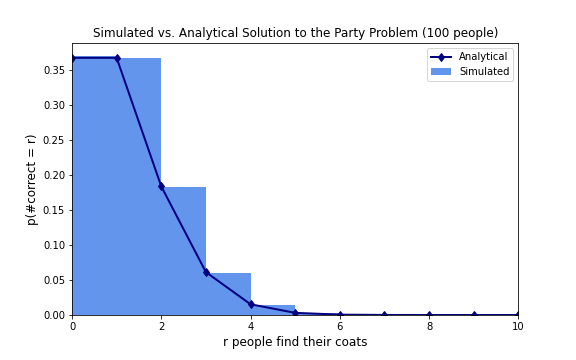
\includegraphics[width=0.7\textwidth]{partyproblem.png}
    \caption{Simulated and analytically calculated probabilities that exactly $r$ people at a $n=100$ people party randomly pick up their coat.}
    \label{fig:proba_partyproblem}
\end{figure}



\section{Copulas}


\section{Relationships Between Distributions}

\section{Large Deviation Theory}
\subsection{Gaertner-Ellis Theorem}
\subsection{Example: Sum of Uniform Random Variables}